\documentclass[12pt,preview]{standalone}
\usepackage[labelfont={bf,sf}]{caption}
\usepackage[verbose,tmargin=1in,bmargin=1in,lmargin=1in,rmargin=1in]{geometry}
\usepackage[T1]{fontenc}
\usepackage{float}
\usepackage{graphicx}
\usepackage{lmodern}
\usepackage{subfig}
\usepackage{amssymb}
%\usepackage{subcaption}
\global\long\def\taxonomy{\mbox{\ensuremath{\mathbb{T}}}}

\global\long\def\prunedTaxonomy{\taxonomy_{P}}

\global\long\def\phyloinputs{\mathcal{T}}

\global\long\def\expandedPhylo{\phyloinputs_{E}}

\global\long\def\summaryTree{\mathbb{S}}

\global\long\def\prunedSummary{\summaryTree_{P}}

\global\long\def\collections{\mathcal{C}}
\begin{document}
\begin{figure}
\subfloat[Input tree $T_{1}$ named ``tree1'']{%
\begin{minipage}[c][1\totalheight][t]{0.25\columnwidth}%
\includegraphics[scale=0.5]{Fig13a}%
\end{minipage}

}\hfill{}\subfloat[Summary Tree $\protect\summaryTree$]{%
\begin{minipage}[c][1\totalheight][t]{0.35\columnwidth}%
\includegraphics[scale=0.5]{Fig13b}%
\end{minipage}

}\hfill{}\subfloat[Induced Tree $\protect\summaryTree(1)$]{%
\begin{minipage}[c][1\totalheight][t]{0.35\columnwidth}%
\includegraphics[scale=0.5]{Fig13c}%
\end{minipage}

}

\bigskip{}

\bigskip{}

\hfill{}\subfloat[JSON annotations relating edges of (c) to edges of (a)]{%
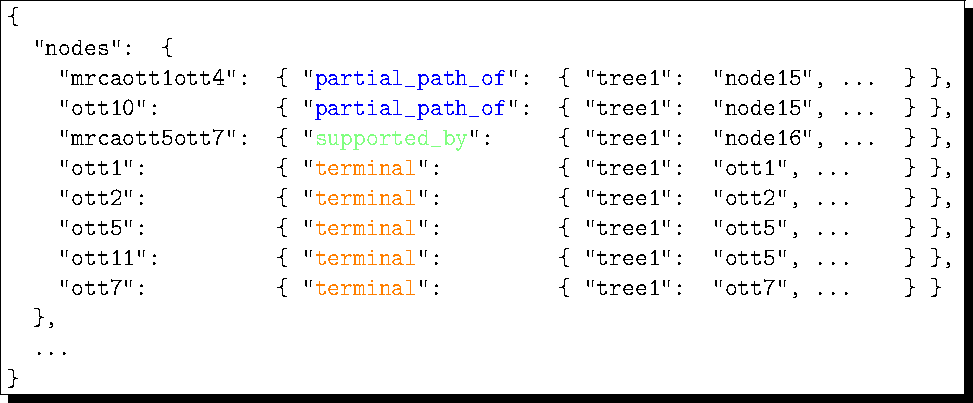
\includegraphics{Fig13d}%
}\hfill{}

\end{figure}
\end{document}